\section{Datenbehandlung}

Aufgrund der Vielfalt der genutzten Datenformate zur Speicherung von Biosignalen und der Nichtexistenz eines einheitlichen Standards \cite{Schlogl2009, Varri2001, Wang2010} muss ein Format gesucht werden, dass zur Behandlung von Datens"atzen im Rahmen dieser Arbeit geeignet ist.
Die Wahl des Datensatzformates st"utzt sich auf die vergleichende Untersuchung \cite{Schlogl2009} von Dr. Alois Schl"ogl der Technischen Universit"at Graz.
Das Unisens-Format besitzt eine Referenzimplementierung mit Programmierschnittstellen sowohl f"ur Matlab als auch f"ur Java und bietet f"ur diese Arbeit optimale Anwendungsvoraussetzungen.
Die Organisation "uber eine menschlich les- und editierbare Headerdatei ist gerade in der Entwicklung interessant.
Es kann ein Datensatz einfach und ohne Bearbeitungstools ver"andert und an die Bed"urfnisse angepasst werden.
Einer der Kritikpunkte nach \cite{Schlogl2009} ist, dass das Format aus mehreren Dateien besteht.
Da die Behandlung von Dateien und Verzeichnissen mit der aktuellen Software kaum noch Unterschiede f"ur den Anwender darstellt, ist nach Meinung des Autors dieser Punkt nicht von hoher Priorit"at.
Es bietet sogar die M"oglichkeit Daten direkt von Sensoren (bei bekannten technischen Parametern wie z.B. Abtastrate und -aufl"osung) direkt in einen Datensatz integriert werden k"onnen.
Zus"atzlich bietet das Format durch seine Definition eine gute Erweiterbarkeit.
Es kann somit an die neue Gegebenheiten und Voraussetzungen angepasst und optimiert werden.

%	-- menschlich editierbar (xml header)
%	-- verzeichnis vs eine datei ist vernachl"assigbar
%	-- reine sensordaten importierbar
%	-- implementierung vorhanden
%	-- f"ur matlab und java

\subsection{Unisens}

Das vom Forschungszentrum Informatik und Institut f"ur Technik der Informationsverarbeitung der Universit"at Karlsruhe entwickelte Datenformat Unisens dient der Speicherung und der Dokumentation von Sensordaten.
Unisens ist konzipiert, Daten verschiedener Sensoren innerhalb eines Datensatzes zu speichern.
Ein Datensatz ist im Dateisystem durch ein eigenes Verzeichnis und eine Headerdatei \verb|unisens.xml| hinterlegt.
In der Headerdatei werden alle Informationen "uber die Bestandteile des Datensatzes, deren Formatierung und ihre semantischen Zusammenh"ange gespeichert.
Messwerte eines Sensors werden "ublicherweise in einer Datendatei innerhalb des Datensatzverzeichnisses abgespeichert.
Eine solche Datendatei wird als \emph{Entry} in dem Datensatz bezeichnet.
Alle Metainformationen zu den Sensordaten werden in der Headerdatei abgspeichert, so dass die Datendateien selbst immer nur die reinen Messdaten enthalten.
Als m"ogliche Sensordaten werden sowohl kontinuierlich abgetastete Signale als auch ereignisorientierte Daten unterst"utzt.
Unisens unterscheidet zwischen vier Arten von Daten:
\begin{description}
	\item[Signale \emph{(Signal)}] \hfill \\
		Signale sind "aquidistant abgetastete, numerische Messdaten.
		Sie zeichnen sich durch eine beliebige aber konstante Abtastrate und Abtastaufl"osung aus.
		Zudem k"onnen Signale aus mehreren Kan"alen bestehen, die alle in ein und derselben Datei abgespeichert werden.
		Alle Kan"ale desselben Signals haben auch dieselbe Abtastrate und -aufl"osung.
	\item[Ereignisse \emph{(Event)}] \hfill \\
		Ereignisse sind diskrete Zeitpunkte die mit einer textlichen Beschreibung versehen sind. (z.B. Triggersignale)
		Sie zeichnen sich durch einen Zeitstempel und einer kurzen Beschreibung aus.
		Optional k"onnen noch Kommentare zu einem Ereignis hinzugef"ugt werden.
	\item[Einzelwerte \emph{(Value)}] \hfill \\
		Einzelwerte sind eine Kombination der beiden oben genannten Datenarten.
		Sie beinhalten numerische Werte die zu bestimmten Zeitpunkten aufgenommen wurden.
		Mit Einzelwerten ist es m"oglich Daten zu speichern, die nicht in festen Zeitintervallen gemessen werden.
	\item[Propriet"are Daten \emph{(Custom data)}] \hfill \\
		Mit dieser Art k"onnen anwendungsspezifisch Daten gespeichert werden, die durch die drei oben genannten Arten nicht erfasst werden k"onnen.
		So k"onnen beispielsweise schematische Darstellungen des Messaufbaus als Bilddateien oder Patienteakten in Form von Textdateien dem Datensatz hinzugef"ugt werden.
\end{description}
Eine detailiertere Beschreibung des Formates kann der offiziellen Dokumentation \cite{Ottenbacher2010} entnommen werden.

\subsubsection{Details der Referenzimplementierung}

In diesem Abschnitt wird kurz auf einige Details der Umsetzung des Unisens-Formates eingegangen.
Das Unisens-Paket ist in Java implementiert und wird unter der \emph{\ac{lgpl}} zur Verf"ugung gestellt.
Die bereit gestellte Bibliothek ist auf zwei Einzeldateien aufgeteilt: \verb|org.unisens.jar| und \verb|org.unisens.ri.jar|.
Bei der ersten Datei handelt es sich um die Definiton des Unisensformates und seiner Bestandteile als Javalassenstruktur.
Diese Definition erfolgt haupts"achlich als \emph{Interface}klassen und legt die Schnittstellen zwischen den einzelnen Bestandteilen fest.
Eine "Ubersicht der Klassenstruktur und der von au\ss en ersichtlichen Attribute ist in \picref{unisens_interface} auf Seite \pageref{pic:unisens_interface} dargestellt.
\begin{sidewaysfigure}%[h]
\centering
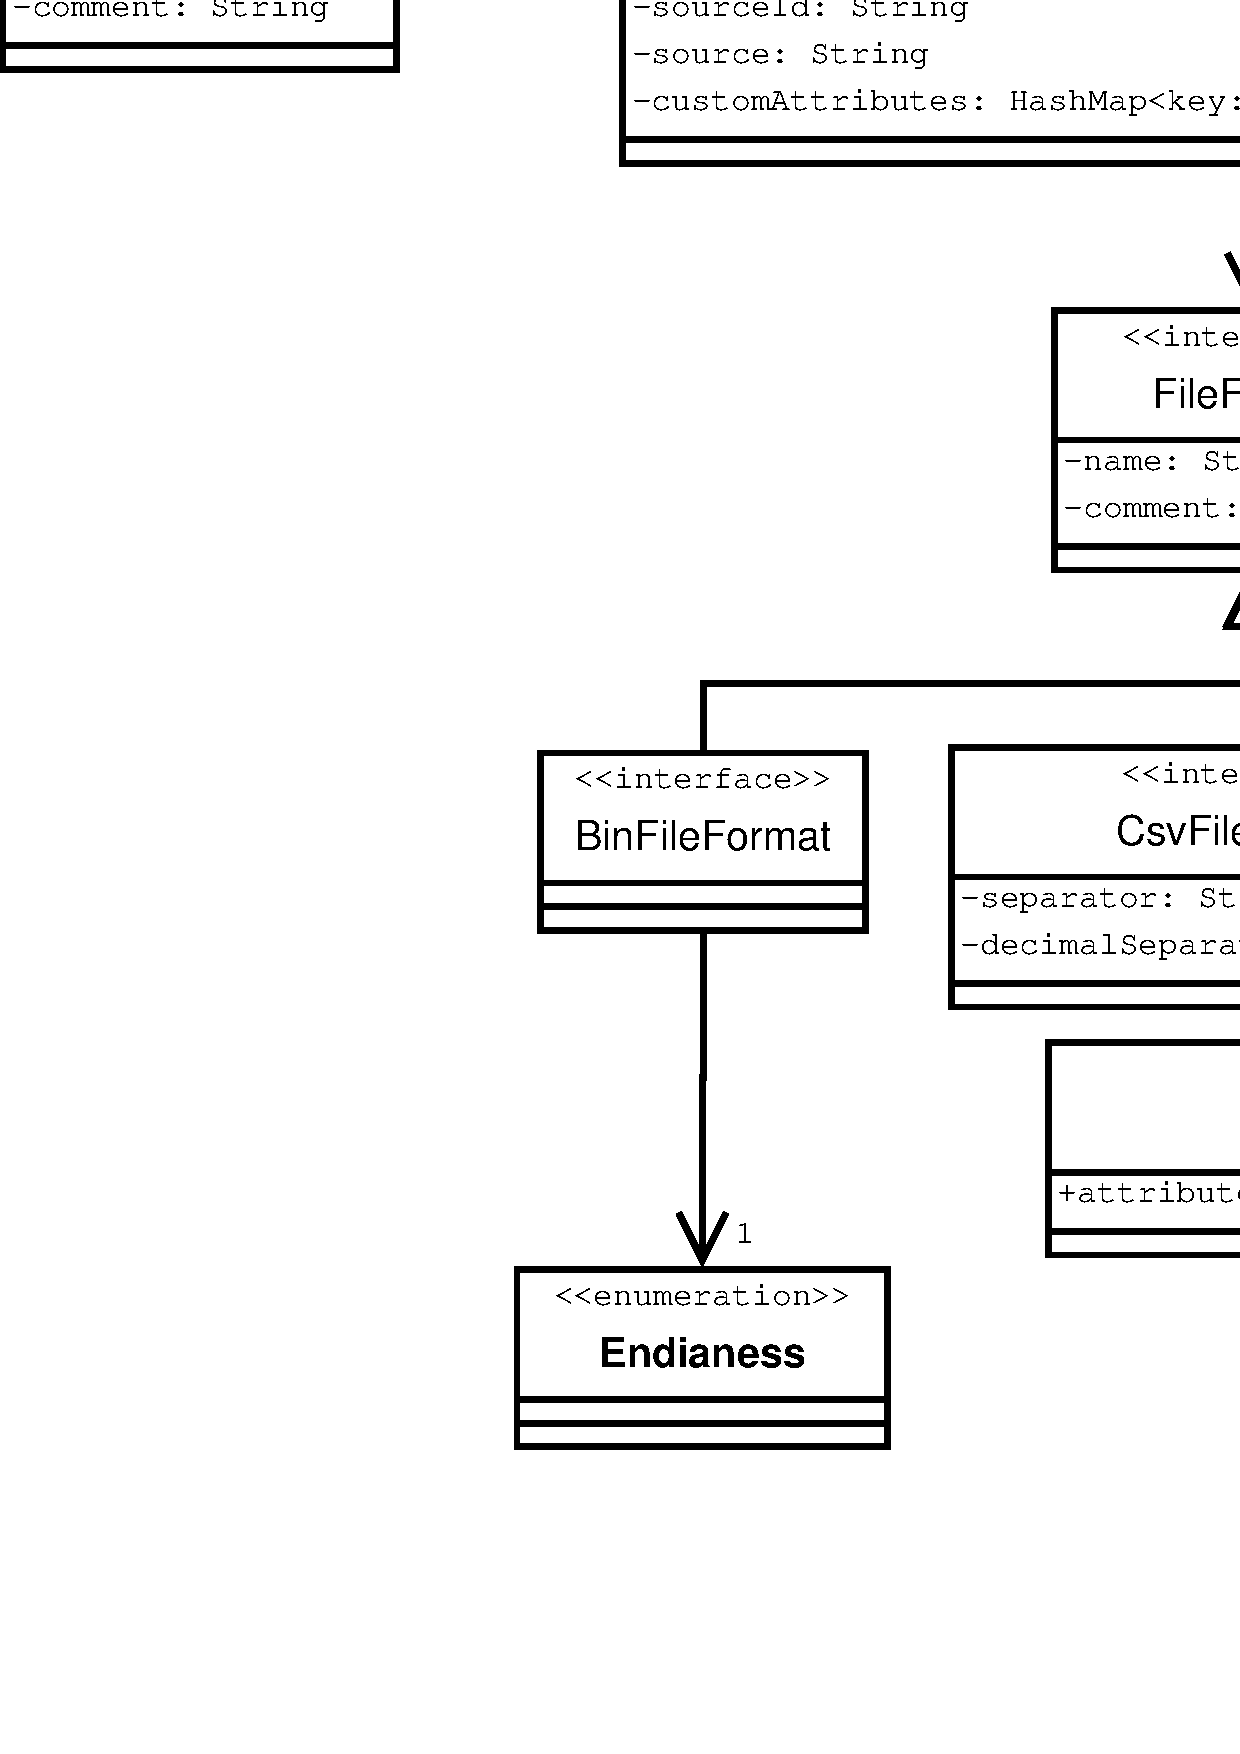
\includegraphics[angle=-90, width=0.9\textwidth]{bilder/unisens_interface_.pdf}
\caption{Klassen"ubersicht der von Unisens definierten Schnittstellen}
\label{pic:unisens_interface}
\end{sidewaysfigure}
Die vom Unisensformat unterst"utzten Signalarten sind auch in der Klassenstruktur in \tabref{unisens_signalklassen} erkennbar.
\begin{table}[h]
\centering
\begin{tabular}{|c|c|}
	\hline Signale & \verb|SignalEntry| \\
	\hline Ereignisse & \verb|EventEntry| \\
	\hline Einzelwerte & \verb|ValuesEntry| \\
	\hline Propriet"are Daten & \verb|CustomEntry| \\
	\hline
\end{tabular}
\caption{Signalarten und ihre repr"asentierenden Klassen}
\label{tab:unisens_signalklassen}
\end{table}

Aufgrund der Ableitung der Klassen \verb|EventEntry| und \verb|ValuesEntry| von \verb|TimedEntry| ist ersichtlich, dass die Zeitpunkte von Ereignisdaten und Einzelwertdaten "uber eine virtuelle Abtastrate bestimmt werden.
Der Zeitpunkt eines jeden \emph{Event}- oder \emph{Value}-Eintrags ist als ganzzahlige Samplenummer dieser Abtastrate gespeichert.
Die Zeit eines Ereignisses, relativ zum Messbeginn, errechnet sich somit $Zeitpunkt = {Samplenummer \over Abtastrate}$.
M"ochte man die M"oglichkeit Ereignisse f"ur jeden beliebigen Datenpunkt eines Datensatzes zuordnen zu k"onnen, dann muss die virtuelle Abtastrate als das kleinste gemeinsame Vielfache aller vorhandenen Abtastraten gew"ahlt werden.

Die Schnittstellendefinition des Unisensformats stellt nur Methoden zum Lesen und Anh"angen von Datenpunkten an den Datensatz bereit.
Somit wird ein Einf"ugen, L"oschen oder Ver"andern von Datenpunkten innerhalb eines Dateneintrags nicht unterst"utzt.
Sollen diese Funktionen vorhanden sein, so muss diese Funktionalit"at selbst implementiert werden.

Die eigentliche Umsetzung der Funktionalit"at ist in der zweiten Datei abgespeichert.
Im Folgenden soll sich der Begriff Referenzimplementierung auf diese funktionelle Umsetzung beziehen.
Die Klassen der Referenzimplementierung bestehen aus den Klassennamen der Schnittstellendefinition und dem Suffix "`Impl"' (z.B. Objekte die den Datensatz darstellen haben die Klasse \verb|UnisensImpl|).
Wenn man schon vorhandene Unisensdatens"atze benutzen m"ochte reicht es aus, die Schnittstellendefinition zu kennen und zu nutzen.
Sollen hingegen konkret Objekte erstellt werden, muss auf die Referenzimplementierung zur"uckgegriffen werden.

Durch einen Fehler in der Referenzimplementierung kann es vorkommen, dass beim Laden eines vorhandenen Unisensdatensatzes in dem Gruppen definiert sind eine \verb|NullPointerException| auftritt.
Insbesondere tritt dieser Fehler auf, wenn innerhalb der Headerdatei der Gruppeneintrag nicht hinter den Dateneintr"agen steht.

\subsection{Programminterne Datenstruktur}

\begin{figure}[htb]
\centering
\includegraphics[angle=-90, width=\textwidth]{bilder/package_data_ubersicht.pdf}
\caption[\acs{uml}-Diagramm des \texttt{data}-Paketes]{\ac{uml}-Diagramm des \texttt{data}-Paketes inklusive der bereitgestellten Schnittstellen}
\label{pic:data_package}
\end{figure}

Das Paket \verb|gst.data| ist die Schnittstelle der Programms zu dem gew"ahlten Datensatzformat Unisens.
Eine "Ubersicht des Paketes ist im \ac{uml}-Diagramm in \picref{data_package} dargestellt.
Dieses Paket erf"ullt zwei wesentliche Aufgaben:
\begin{itemize}
	\item Vereinheitlichung der Behandlung der unterschiedlichen Datenarten
	\item Abkapselung anderer Programmteile vom Datensatzformat
\end{itemize}

Die Vereinheitlichung ist notwendig, da Unisens die Daten in drei Arten gliedert: Signale, Werte und Ereignisse.
F"ur die Bearbeitung und Darstellung ist aber die Unterscheidung von Signalen und Werten nicht notwendig.
In beiden F"allen handelt es sich um numerische Werte die zu einem bestimmten Zeitpunkt aufgenommen wurden.
Somit sollen diese auch vom Programm gleichartig behandelt werden.
Daher erhalten alle Datenarten die abstrakte Klasse \verb|DataController| als Fassade.
Die jeweilge konkrete Implementierung ist in den drei abgeleiteten Klassen \verb|Signal-|, \verb|Value-| und \verb|AnnotationController| realisiert.
Neben der Vereinheitlichung der Schnittstelle zum Datensatz werden auch die Zugriffe auf die Daten vereinfacht.
Es werden notwendige Ausnahmebehandlungen (\emph{Exceptions}) durch die Klassen des \verb|data|-Paketes abgefangen und behandelt.
Darunter f"allt unter anderem die Behandlung von Fehlern, wenn Daten aufgrund von fehlenden Zugriffsrechten nicht gelesen oder geschrieben werden k"onnen.
Somit ist der Zugriff auf die konkreten Daten des Datensatzes sowohl vereinheitlicht als auch vereinfacht.

Weiterhin wird mit dem \verb|data|-Paket erreicht, dass die restlichen Komponenten des Programms nicht direkt auf das Datensatzformat zugreifen.
Sie sind damit von dem gew"hlten Format abgekapselt und ein Austausch des Formates erfordert nur die Anpassung des \verb|data|-Paketes.
Der gesamte Datensatz ist durch die Wrapper-Klasse \verb|UnisensDataset| im Programm repr"asentiert.
Zugriff auf den Datensatz erfolgt nur "uber die von der Klasse bereitgestellte Schnittstelle.
Weiterhin wird der ver"anderde Zugriff auf Annotationen durch die Klasse \verb|AnnotationManager| realisiert und die Behandlung von Annotationen selbst "uber die Klasse \verb|AnnotationList| abgewickelt.
Die zwei zu letzt genannten Klassen kapseln die von Unisens bereitgestellten Klassen (\verb|Event| und \verb|EventList|) von den anderen Programmteilen ab.

Neben den zwei oben genannten Aspekten wird auch der Zugriff auf die Daten selbst durch das Paket ver"andert.
Unisens arbeitet durchgehend mit Samplenummern bei der Indizierung der einzelnen Datenpunkte.
Die durch das Paket bereitgestellte Schnittstelle wandelt diese Art des Zugriffs auf eine zeitbasierte Art um.
Das bedeutet, anstatt Daten "uber die Angabe von Samplenummern zu erhalten, bietet die Schnittstelle die M"oglichkeit Daten aus einem bestimmten Zeitraum zu erhalten.
Die notwendige Umrechnung zwischen Samplenummern und Abtastraten auf entsprechende Zeitpunkte wird im \verb|data|-Paket ausgef"uhrt.
Dadurch wird die Existenz verschiedener Abtastraten der unterschiedlichen Signale vor dem restlichen Programm verborgen.

\subsubsection{Repr"asentation des Datensatzes durch die Klassen \texttt{UnisensDataset} und \texttt{DataController}}

Die Klasse \verb|UnsiensDataset| stellt die Schnittstelle des Programms zu den Datens"atzen dar.
F"ur jeden geladenen Datensatz wird im Programm ein Objekt der Klasse \verb|UnisensDataset| erzeugt.
Diese Objekte bieteten die erforderlichen Funktionen um auf die Eigenschaften des Datensatzes, die Eigenschaften der Dateneintr"age und die Daten der Eintr"ge selbst zuzugreifen.
Beim Laden eines Datensatzes wird f"ur jeden Dateneintrag ein Instanz eines \verb|DataController|s erzeugt und in einer Liste \verb|ctrlList| im \verb|UnisensDataset|-Objekt gespeichert.
Je nach Datenart des Eintrags wird zur Laufzeit dynamisch ein Objekt der Klassen \verb|Signal-|, \verb|Value-| oder \verb|AnnotationController| erzeugt.
Genauer wird sogar f"ur jeden Kanal ein eigener \verb|DataController| angelegt.
Jede Komponente des Programms die auf einen Dateneintrag zugreifen m"ochte, erh"alt vom \verb|UnisensDataset| den entsprechenden Controller.
Es wird sichergestellt, dass zu jedem Zeitpunkt jedem Dateneintrag genau ein Controllerobjekt zugeordnet ist und keine Duplizierung auftreten kann.
Durch spezielle Funktionen \verb|AddNewSignal()|, \verb|AddNewValue()| und \verb|AddNewAnnotation()| k"onnen einem Datensatz zus"atzliche Dateneintr"age hinzugef"ugt werden.
Die entsprechenden \verb|DataController| werden dann in die Liste \verb|ctrlList| aufgenommen und es kann durch diese anschlie\ss end auf die Daten zugegriffen werden.
Der gesamte Datensatz wird bei einem Aufruf der \verb|save()|-Funktion des Datensatzes abgespeichert werden, weil die Speicherfunktion f"ur alle \verb|DataController|-Objekte in \verb|crtlList| rekursiv ausgef"uhrt werden k"onnen.

\subsubsection{[WIP]Das Singleton-Konzept und \texttt{DatasetList}}

\begin{figure}[htb]
\centering
\includegraphics[angle=-90, width=0.8\textwidth]{bilder/singleton_datasetlist.pdf}
\caption{Klasse \texttt{DatasetList} und das Singleton-Konzept}
\label{pic:datasetlist}
\end{figure}

- \picref{datasetlist}
- alle DS in einer einzigartigen Liste zusammengefasst
- Singleton Konzept erkl"aren \cite{Gamma1995} (Seiten 127 bis 134)
- stellt sicher, dass jeder DS nur einmal geladen wird

\subsubsection{Pufferung, Sortieren und Suchen der Klasse \texttt{AnnotationController}}

Die Referenzimplementierung des Unisensformates sieht f"ur das Lesen und Schreiben von Daten einen ungepufferten Ansatz vor.
Das bedeutet sobald Daten vom Programm ver"andert werden, werden diese "Anderungen auch sofort im Datensatz und somit auf dem Speichermedium abgespeichert.
Das hat zur Folge, dass Annotationen in der Reihenfolge in der sie erstellt wurden, in den Datendateien abgespeichert werden.
Somit sind die Annotationen zeitlich unsortiert.
Wenn nun eine Annotation eines bestimmten Zeitpunktes angezeigt werden soll, muss der im schlechtesten Fall der gesamte Datensatz nach dieser Annotation durchsucht werden.
Dieses Verhalten ist unerw"unscht, da somit die Zugriffszeit w"ahrend der Laufzeit, insbesondere bei gro\ss en Datens"atzen, stark schwanken k"onnen.
Dieses Problem wird durch eine gepufferte Implementierung der Klasse \verb|AnnotationController| behoben.
Die Annoationen werden beim Laden des Datensatzes in den Arbeitspeicher geladen und mit einem Quick-Sort-Algorithmus nach aufsteigenden Samplenummern sortiert.
Neu erstellete Annotationen werden in dieser Liste an den entsprechenden Stellen einsortiert.
Es wird immer die Samplenummer der Annotation gespeichert, auf die als letztes zugegriffen wurde (sowohl Lesen als auch Schreiben).
Bei der Suche nach der entsprechenden Position einer gesuchten Annotation wird dann von dieser gespeicherten Samplenummer aus gestartet.
Die Suche nach einer Samplenummer erfolgt sowohl vor- als auch r"uckw"arts.
Dieser Ansatz hat den Vorteil, dass eine gesuchte Position nach wenigen Suchschritten erreicht wird, da Annotationen durch den Benutzer nur ver"andert werden k"onnen die auch angezeigt werden.
Somit befindet sich der Index des letzten Zugriffs immer in der N"ahe der gesuchten Position.

\paragraph[{[WIP]Anmerkung zur Quick-Sort-Implementierung}]{[WIP]Anmerkung zur Quick-Sort-Implementierung:}
%\addcontentsline{toc}{paragraph}{Anmerkung zur Quick-Sort-Implementierung}

- w"ahrend der Test und Nutzung ist ein Stack-Overflow aufgetreten bei ca. \unit{3.000} - \unit{3.600} Annotationen
- = zuviele ineinander verschachtelte Funktionsaufrufe
- liegt in der rekursiven Struktur des Sortieralgorithmuses
- konnte mit Vergr"o\ss erung des Stacks "uber den Parameter \texttt{-Xss2m} von \unit{512}{kB} auf \unit{2}{MB} angehoben werden
- Probleme bestehen weiterhin, kann wiederum erh"oht werden auf maximal ??? (gro{\ss}e Datens"atze!)

% newline wegen overfuill box
\subsubsection{[WIP]Direkter Zugriff auf Werte mit der Klasse\newline \class{BufferedValueController}}

- weil Unisens kein gezieltes Einf"ugen von Daten erlaubt
- direkter/wahlfreier Zugriff (\emph{random access}) auf die Daten
- Subklasse \class{DataPoint}
- anderer Ansatz als in \class{AnnotationController}: Daten werden schon beim Lesen in den Puffer einsortiert
- Speichern durch neu schreiben der Datei (alte Datei wird als backup kopiert)

\subsubsection{[WIP]Observer Prinzip zur Reaktion auf Daten"anderung}

- Erkl"arung der Prinzipes \cite{Gamma1995} (Seiten 293 bis 303)
- Observer wird von interessierten Klassen mit der Implementierung des Interface \class{DataChangeListener} realisiert
- die Funktionalit"at ist in der Klasse \class{DataController} implementiert
- Subklassen erzeugen die \class{DataChangeEvent}-Objekte und starten den Ablauf mit dem Funktionsaufruf \texttt{notifyListeners(DataChangeEvent)}
- Bild!

\subsubsection{[WIP]Tests des \texttt{data}-Paketes}

% EOF
